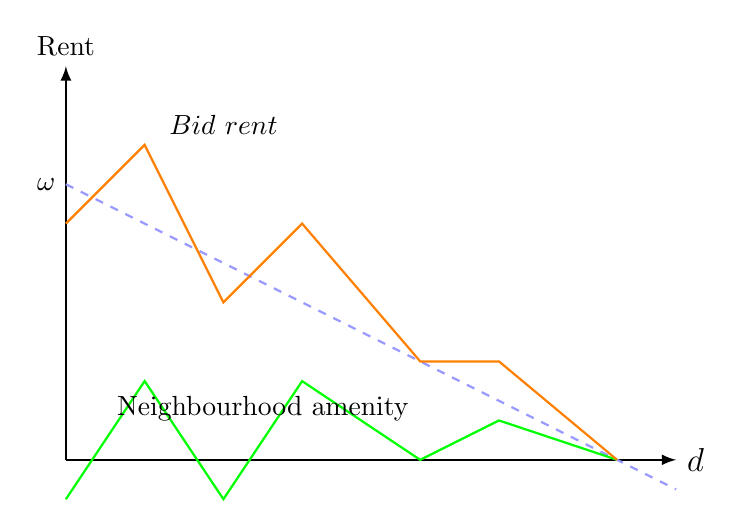
\begin{tikzpicture}[scale=.5]
\def\bndmax{5}        %https://tex.stackexchange.com/questions/68462/filling-a-complex-region-with-tikz
\def\bndmin{0.2}
\def \n {10}
\def \m {15.5}
\def \t {.5}
\def \th {1}
\def \w {7}
\tikzset{func/.style={thick,dashed, color=blue!40}}	
\draw [thick, latex-] (0,\n)node[above] {Rent}--(0,0);
\draw [thick, -latex] (0,0)--(\m,0)node[right=.25]{\large $d$};
% Basic Bid rent,
\node at(-.5,\w) {$\omega$};
\draw[func,domain=0:\m] plot [samples=200] (\x,{\w-\t*\x});
%NEIGBOURHOOD AMENITY
\draw [thick, green] (0,-1)--(2,2)--(4,-1)--(6,2)--(9,0)--(11,1)--(14,0);
\draw [thick, orange] (0,6)--(2,{7-2*.5+2})--(4,7-4*.5 -1)--(6,7-6*.5+2)--(9,7-9*.5)--(11,7-11*.5+1)--(14,7-14*.5);
\node [] at (5,1.3){Neighbourhood amenity};
\def \azero{2}
\def \aprime {-.25}	
% \tikzset{func/.style={thick,color=orange!90}}	
% 	\draw[func,domain=0:\m] plot [samples=200] (\x,{\w+\azero-\t*\x+\aprime*\x});
\node at (4,8.5){$Bid\ rent$};
%\node at(-.8,2) [left]{base $2^1=$};
%\node at(-.8,1) [left]{$2^0=$};
%\draw[dotted] (0,2)--(1,2)--(1,0); 
 \end{tikzpicture}